\section{Active Circuit Elements}
\subsection{HF Diodes}
\subsubsection{Schottky Diodes}
\begin{itemize}
    \itemsep0pt
    \item n-type semiconductor; better carrier mobility of electrons
    \item Small barrier capacitance $\implies$ \textit{Fast switching}
    \begin{equation*}
        \text{Characteristic curve: }i = I_0 \left(\mathrm{exp}\left(\dfrac{u}{U_T} - 1\right)\right)
    \end{equation*}
\end{itemize}

\subsubsection{Capacitance/Varactor Diode}
\begin{itemize}
    \itemsep0pt
    \item Reverse biased p-n-diode; application of reverse voltage causes a barrier
    \item Increasing voltage $\to$ decreasing capacitance
    \item Can be used as an \textit{electronically variable capacitance}
    \item \textbf{Application:} tuning of resonators, filters, ...
\end{itemize}

\subsubsection{Tunnel Diode}
\begin{itemize}
    \itemsep0pt
    \item The u-i-characteristic exhibits regions with \textit{negative differential resistance}
    \item Can be used for the \textit{amplification of high-frequency} signals
    \item \(G_{n} \downarrow \left(|U|\uparrow \right)\)
\end{itemize}

\subsubsection{Impatt Diode}
\begin{itemize}
    \itemsep0pt
    \item Written out: \textbf{imp}act ionization \textbf{a}valanche \textbf{t}ransit \textbf{t}ime
    \item Negative differential resistance
    \item Usage in high-power applications
    \item Amplifier/Oscillator
    \item \textbf{Drawback:} high phase noise from avalanche effect
    \item Operation as a \textit{read diode}:
        \begin{align*}
            \Theta = \omega t = \omega \; w/v_s\\
            I_D = I_{\mathrm{max}} \dfrac{\Theta}{\pi} e^{-j\Theta/2} \dfrac{\sin\Theta/2}{\Theta/2}
        \end{align*}
    \item \(R_n \downarrow \left(|U_s|\uparrow\right)\)
    \item Operation up to \SI{94}{GHz}
\end{itemize}

\subsubsection{PIN Diode}
\begin{itemize}
    \itemsep0pt
    \item \textit{Positive-intrinsic-negative} diode
    \item Constant charge can be achieved by impressing a current \(|I_{DC}| = \left|\dfrac{dQ_x}{dt}\right|\)
    \item Properties:
        \begin{itemize}
            \itemsep0pt
            \item Fast switching times between high resistance and short circuit \(\approx \SI{1}{ns}\)
            \item linearly variable HF resistance
            \item Low insertion loss
            \item High break-through voltage due to large length of intrinsic zone possible
        \end{itemize}
    \item Use cases:
        \begin{itemize}
            \itemsep0pt
            \item Electronic switching element
            \item Variable $\pi$-attenuator with input-output matching to a real wave impedance
        \end{itemize}
\end{itemize}


\subsubsection{Gunn Element}
\begin{itemize}
    \itemsep0pt
    \item The Gunn Element is \textit{not} a diode
    \item Oscillator/Amplifier
    \item \textbf{Justification:} \textit{negative differential mobility} of the electrons (negative resistance/conductance)
\end{itemize}

\subsection{HF-Transistors}
\fbox{%
    \parbox{8cm}{%
        \textbf{Two-step analysis of HF-Transistor Amplifier Circuits:}
        \begin{enumerate}
            \itemsep0pt
            \item DC-analysis around quiescent point $\implies$ calculate resistances
            \item Small signal analysis using HF equivalent circuit
        \end{enumerate}
    }
}
\subsubsection{Bipolar Transistor}
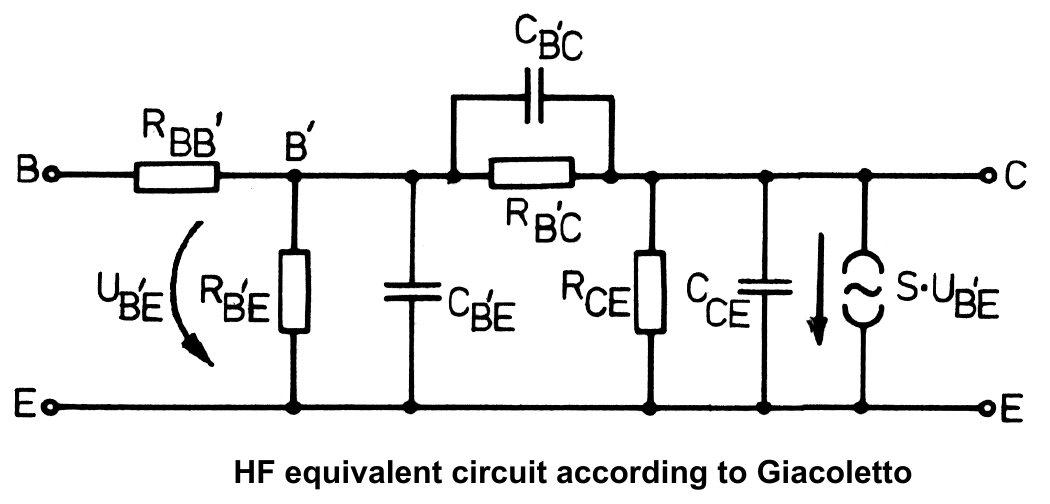
\includegraphics[width=.3\paperheight]{content/hfcomp/pictures/bipolar_transistor_giacoletto.png}
\begin{align*}
    &S \approx \dfrac{I_{E,DC}}{U_T}, \quad C_{B^\prime E} \approx \dfrac{S}{2\pi f_T},\\
    &\dfrac{1}{R_{B^\prime E}} = G_{B^\prime E} \approx \dfrac{S}{\beta_0},\\
    &\beta_0 = \left.\dfrac{I_C}{I_B}\right|_{f\to0} \approx \dfrac{I_{C,DC}}{I_{B,DC}} = B,\\
    &U_T = \frac{k_B T}{q_e}, \; U_T(T=\SI{25}{\degree C}) \approx \SI{25}{mV}\\
    &f_T\text{: transit frequency }(\beta = 1),\\
    &B\text{: DC current amplification},\\
    &k_B\text{: Boltzmann constant},\\
    &T\text{: Abs. temperature in Kelvin},\\
    &q_e\text{: Elementary charge}
\end{align*}
\begin{itemize}
    \itemsep0pt
    \item The HF operational parameters depend on the chosen operating point. The following is also achieved:
    \begin{itemize}
        \itemsep0pt
        \item \textit{Control} and \textit{stabilization} of the HF operational parameters
        \item Compensation of \textit{device tolerances}
        \item \textbf{Principle:} DC current feedback circuit
    \end{itemize}
\item E12-series resistors:
    \begin{equation*}
        R_n = 10^\frac{n}{12} 10^p \quad n=0,1,2,...
    \end{equation*}
\end{itemize}

\subsubsection{Field-effect Transistor}
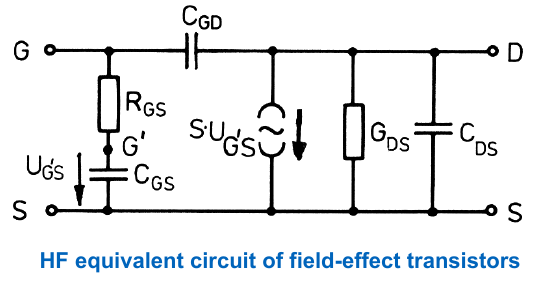
\includegraphics[width=.3\paperheight]{content/hfcomp/pictures/mosfet_hf_equivalent.png}\\
n-channel MOSFET, depletion type:
\begin{align*}
    &i_D \approx I_{DSS} \left(1 - \dfrac{u_{GS}}{U_P}\right)^2\\
    &S = \left.\dfrac{\partial i_D}{\partial u_{GS}}\right|_{U_{DS}=\mathrm{const}} = \dfrac{2}{|U_P|}\sqrt{I_{DSS} \; i_D}\\
    &U_P\text{: pinch-off voltage, here } U_P < 0
\end{align*}

\subsection{Microwave Tubes}
\subsubsection{Klystron}
\begin{itemize}
    \itemsep0pt
    \item Continuous electron beam is velocity modulated by an HF signal $\implies$ density-modulation
    \item Density modulated beam equivalent to an AC current $\implies$ excites \textit{amplified} oscillation in output resonator
\end{itemize}
\begin{align*}
    &i \approx I_0 \left(1 + p \cos(\omega t_0)\right)\\
    &p = \dfrac{\omega l |U_e|}{2v_0 U_0}\text{ (bunching parameter)}
\end{align*}

\subsubsection{Travelling Wave Tube (TWT)}
\begin{itemize}
    \itemsep0pt
    \item Density modulated electrons, as with Klystron
    \item Energy transfer \textit{only if}(!) average electron velocity $v_0$ is greater than the phase velocity $v_p$ of the RF wave $\implies$ delay lines for RF wave
\end{itemize}
\begin{align*}
    &v_p \approx c_0 \sin \psi, \quad v_p < v_0\\
    &\psi\text{: angle of helical delay line}
\end{align*}

\subsubsection{Magnetron (ger.: Kreuzfeldröhre)}
\begin{itemize}
    \itemsep0pt
    \item Similar to Klystron and TWT, but additionally \textit{shaped by DC magnetic field}
    \item Electron beam excites resonators embedded in the cathode
\end{itemize}
